\documentclass[12pt, a4paper]{article}
\usepackage{graphicx}
\usepackage{xurl}
\usepackage{geometry}
\usepackage{float}
\usepackage{indentfirst}
\geometry{left=2.54cm, right=2.54cm, top=3.18cm, bottom=3.18cm}
% \setlength{\parindent}{0pt}

\title{Weekly Reports}
\author{Jerry Jin}

\begin{document}

\maketitle

\section*{Week 10/1 - 10/16}

\subsection*{Goal}

\noindent
Main Task: Establish a basic recurrent neural network!

\begin{itemize}
    \item Get the code from Ankit
    \item Change the acitivation function to sigmoid, and change the synaptic modulation to gain modulation using back-propagation
    \item Simulate sin wave
    \item Simulate Mackey-Glass equation
    \item Obey Dale law
\end{itemize}

\noindent
Reading

\begin{itemize}
    \item Sussillo, D., \& Abbott, L. F. (2009). Generating Coherent Patterns of Activity from Chaotic Neural Networks. Neuron, 63(4), 544–557. \url{https://doi.org/10.1016/j.neuron.2009.07.018}
    \item Nicola, W., \& Clopath, C. (2017). Supervised learning in spiking neural networks with FORCE training. Nature Communications, 8(1), 2208. \url{https://doi.org/10.1038/s41467-017-01827-3}
    \item Maass, W., Natschläger, T., \& Markram, H. (2002). Real-Time Computing Without Stable States: A New Framework for Neural Computation Based on Perturbations. Neural Computation, 14(11), 2531–2560. \url{https://doi.org/10.1162/089976602760407955}
    \item \url{https://en.wikipedia.org/wiki/Reservoir_computing}
\end{itemize}

\newpage

\subsection*{Model}
\begin{itemize}
    \item Structure: 1 input layer (1D input), 1 recurrently-connected hidden layer (128 nodes), 1 output layer (1D output).
    \item Activation function: sigmoid function $r_i = \frac{1}{1 + e^{-g_i(I_i-s_i)}}$, where $I_i$ is the input, $r_i$ is the output, $g_i$ is the gain, $s_i$ is the shift. 
    \item Initialization: input weights, internal weights, output weights, gains, and shifts are randomly initialized using Gaussian distribution. Initial activations are initialized as 0.
    \item Dale's law: specify a proportion of neurons to be excitatory (here 50\%) and others to be inhibitory. excitatory neurons can only have positive weights and inhibitory neurons can only have negative weights.
    \item Tasks:
    \begin{enumerate}
        \item Predict sine wave: $f(t)=sin(at)$, $a=\frac{1}{60\pi}$. Input $f(t)$, train RNN to predict $f(t+1)$.
        \item Predict Mackey-Glass equation: $\frac{d}{dt}g(t)=\frac{\beta_0 g(t-\tau)}{1+g(t-\tau)^n}-\gamma g(t)$, 
        
        $\gamma=0.1, \beta_0=0.2, n=10, \tau=20$. Input $g(t)$, train RNN to predict $g(t+1)$.
    \end{enumerate}
    \item Training: 
    \begin{enumerate}
        \item Gradient descent to update gains and shifts only (SGD optimizer in PyTorch, learning rate=$0.2$).
        % \item Gradient descent on gains and shifts + basic Hebbian learning to update the internal weights ($w_{ij} \rightarrow w_{ij} + \eta r_i r_j$, normalize, $\eta=0.01$ with expnential decay).
        \item Gradient descent on gains and shifts + Oja's learning rule to update the internal weights ($w_{ij} \rightarrow w_{ij} + \eta (r_i r_j - \alpha r_j^2 w_{ij})$, only on weights from excitatory neuron, $\alpha = \sqrt{128}$, $\eta=0.01$ with expnential decay).
    \end{enumerate}


\end{itemize}

\subsection*{SGD on Gains and Shifts Only}

\begin{figure}[H]
    \centering
    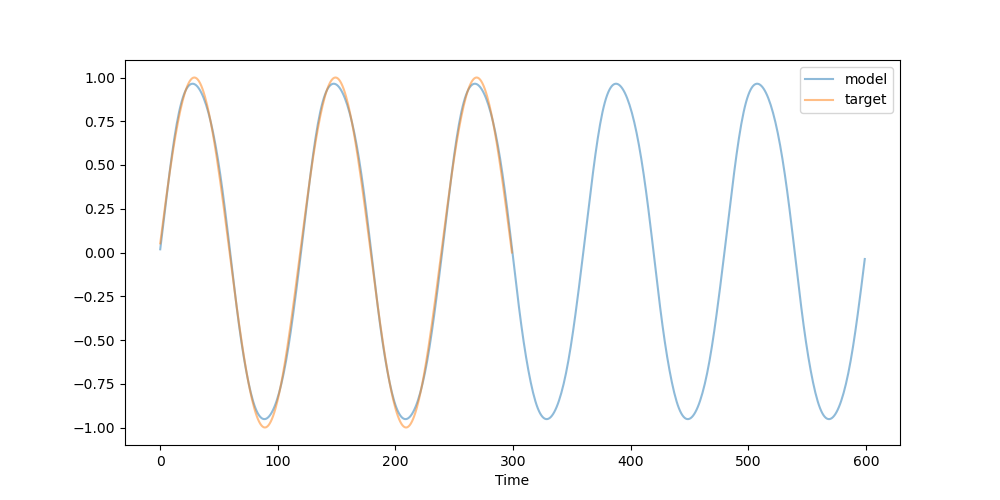
\includegraphics[width=\textwidth]{analysis/fig/1016_SIN_bpgain_output.png}\\
    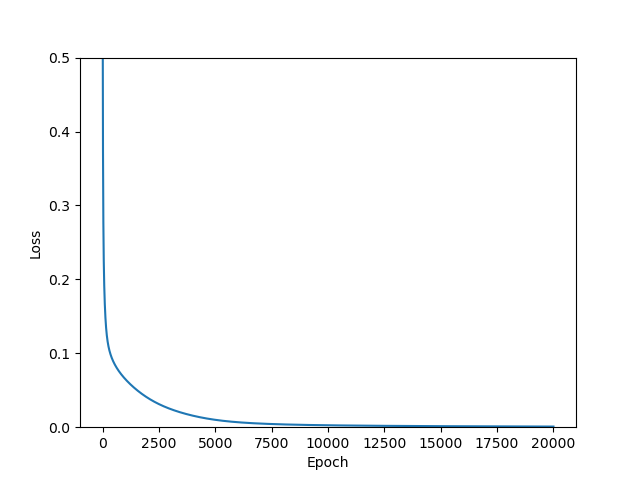
\includegraphics[width=\textwidth]{analysis/fig/1016_SIN_bpgain_loss.png}
    \caption{SIN, SGD only.}
\end{figure}

\begin{figure}[H]
    \centering
    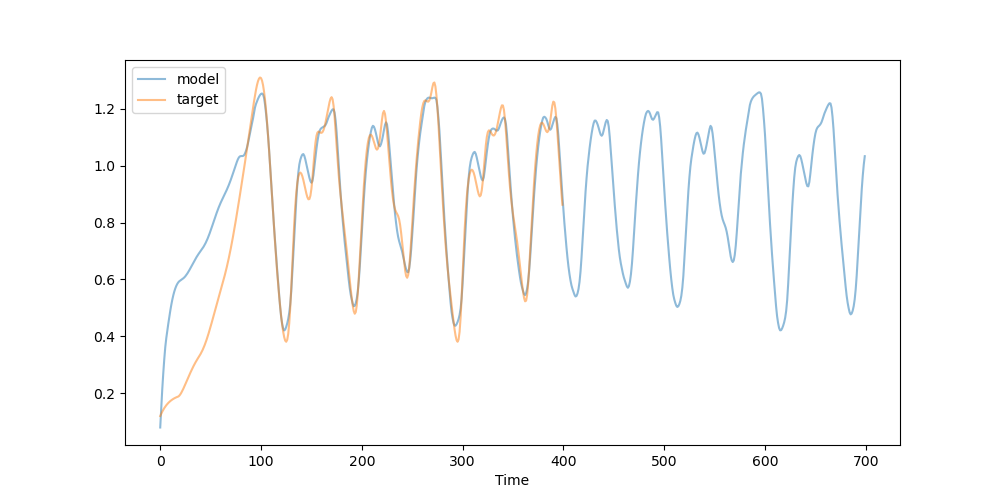
\includegraphics[width=\textwidth]{analysis/fig/1016_MG_bpgain_output.png}
    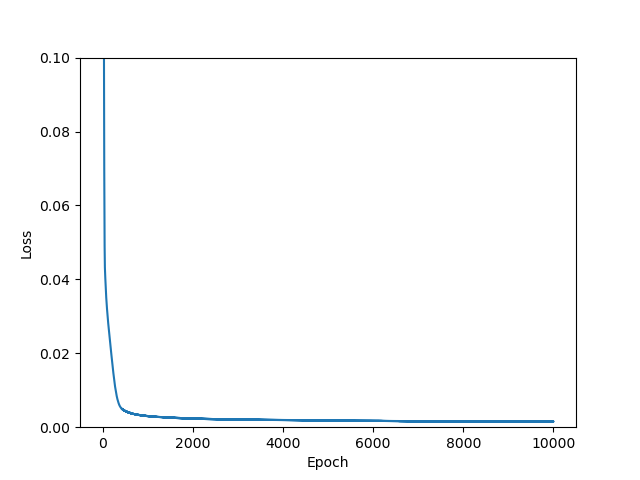
\includegraphics[width=\textwidth]{analysis/fig/1016_MG_bpgain_loss.png}
    \caption{MG, SGD only.}
\end{figure}

Training the RNN with gain modulation while keeping the input matrix, internal matrix, and output matrix as random could approximate sine wave and Mackey-Glass equation, and in the meanwhile obeying the Dale's law.

\subsection*{SGD on Gains and Shifts with Oja's Learning}

For Oja's learning plus gradient descent, it only works when it is with Adam optimizer, not the normal SGD optimizer.

\newpage

%%%%%%%%

\section*{Week 10/16 - 10/31}

\subsection*{Goal}

\noindent
Main Task: Feedback control to Linear RNN, and test the performance under noise.

\begin{itemize}
    \item Add gaussian noise
    \item Add Kalma filter and LQR control signal
\end{itemize}

\noindent
Reading

\begin{itemize}
    \item Charles, A. S., Balavoine, A., \& Rozell, C. J. (2016). Dynamic Filtering of Time-Varying Sparse Signals via $\ell _1$ Minimization. IEEE Transactions on Signal Processing, 64(21), 5644–5656.
    \item Rubin, R., Abbott, L. F., \& Sompolinsky, H. (2017). Balanced excitation and inhibition are required for high-capacity, noise-robust neuronal selectivity. Proceedings of the National Academy of Sciences, 114(44).
    \item Zhang, Z., \& Fujisaki, Y. (2023). Sparse Feedback Controller: From Open-loop Solution to Closed-loop Realization (arXiv:2303.15175). arXiv.
\end{itemize}

\newpage

\subsection*{Model}
\begin{itemize}
    \item Structure: 1 input layer (1D input), 1 recurrently-connected hidden layer (32 nodes) where 50\% are excitatory neurons (obeying Dale's law), 1 output layer (1D output). 

    \item Activation function: for now $y=x$ to make it a simple linear system.
    
    \item Equations: 
    \begin{eqnarray}
    \nonumber
    \dot{x_t} = (W-I)x_t + I_{t} + u_{t} + w_d \\
    \nonumber
    y_t = Cx_{t} + w_n
    \end{eqnarray}
    
    \item $x_t$ is the activation, $I_t$ is the input after input layer, $u_t$ is the control input, $w_d$ is the Gaussian processing noise following $N(0,W_d)$, $w_n$ is the Gaussian measurement noise following $N(0,W_n)$, $W$ is the weight matrix, $C$ is set to be identity matrix.

    \item In the absense of control input and noise, use backpropagation to train the weight matrix $W$ so that $x_t$ gives ideal outputs after output layer. We refer to such $x_t$ as reference activations $r_t$.

    \item Kalman filter: $\dot{\hat{x}_t} = (W-I)\hat{x}_t + I_{t} + u_{t} + K_f(y_t - C\hat{x}_t)$.
    
    \item LQR: $u_t = -K(\hat{x}_t - r_t)$, to minimize $\int x^TQx + u^TRu \,dt$.

    \item For SIN, $Q = I$, $R = 0.01I$, $W_d = 0.01I$, $W_n = 0.001I$. For MG, $Q = I$, $R = 0.1I$, $W_d = 0.001I$, $W_n = 0.0001I$. These choices, as well as the number of nodes, may influence convergence.

\end{itemize}

% structure plot!
\begin{figure}[H]
    \centering
    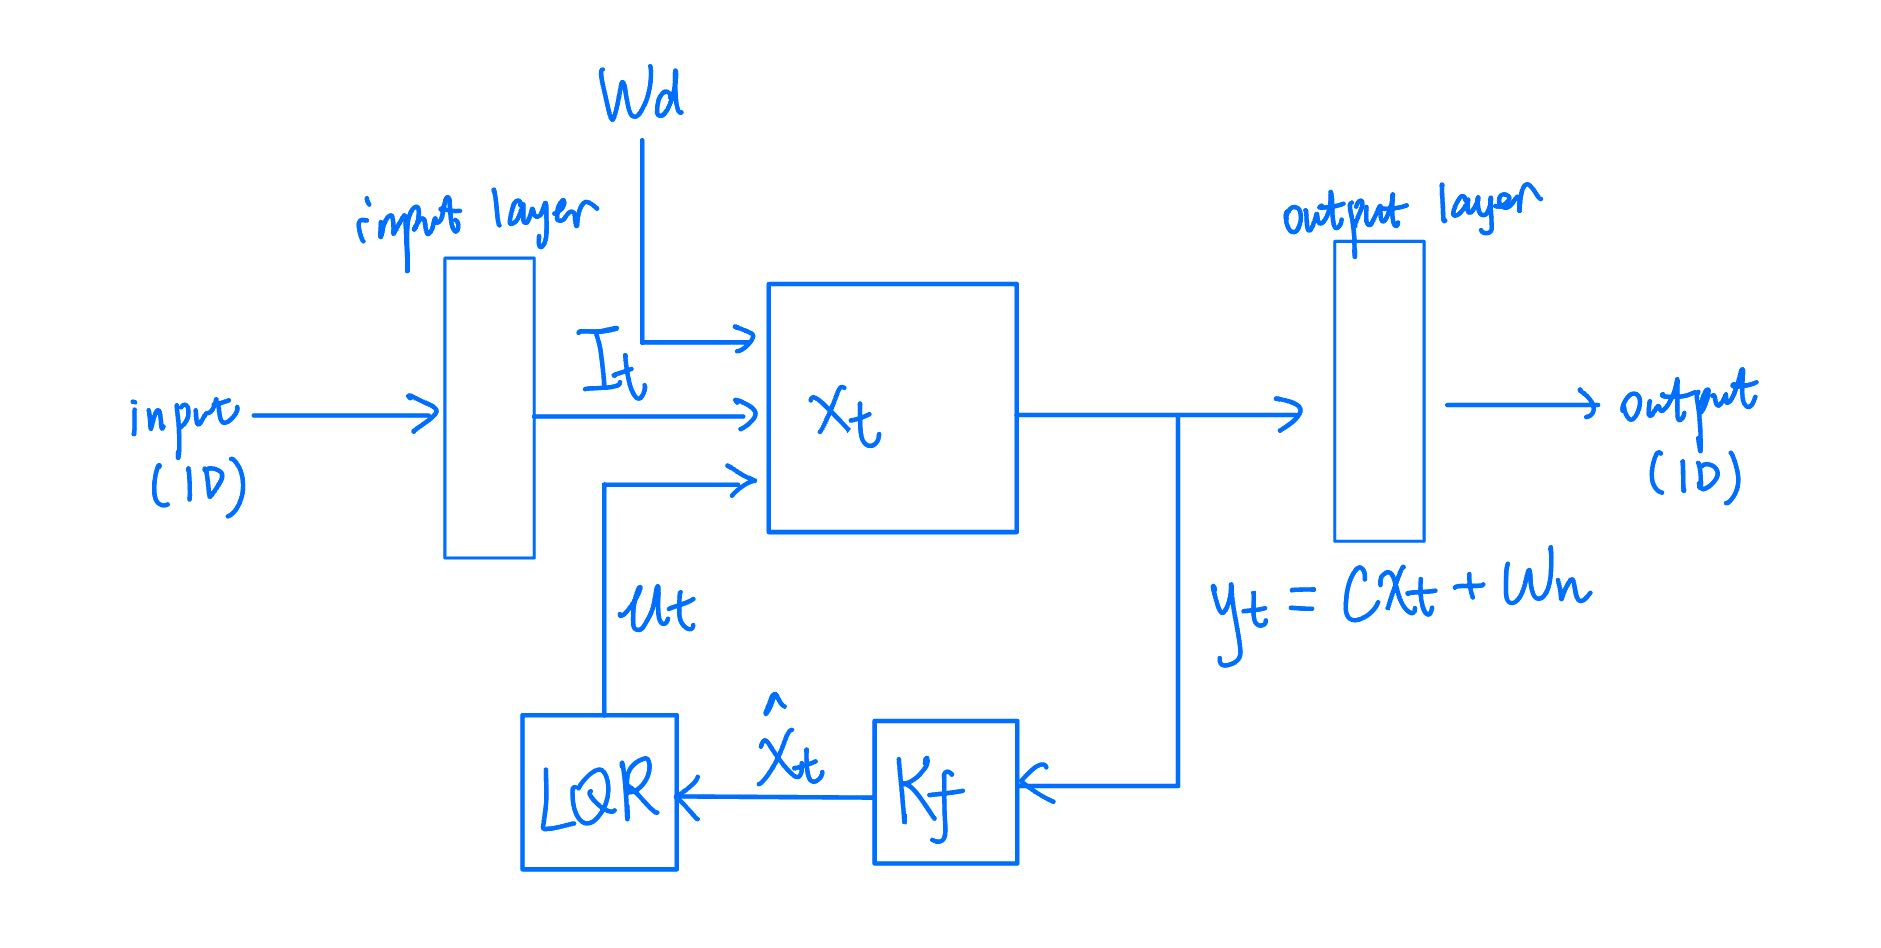
\includegraphics[width=0.9\textwidth]{baseline_linear/fig/lqg_structure.jpg}
\end{figure}

\subsection*{Persistent and Instant Perturbation}

\begin{figure}[H]
    \centering
    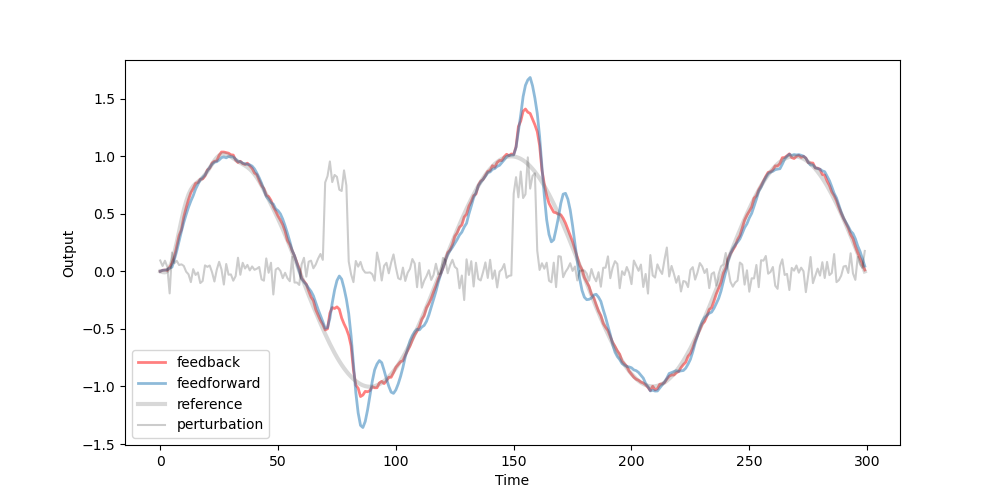
\includegraphics[width=\textwidth]{baseline_linear/fig/SIN_lin_noise.png}
    \caption{SIN, linear RNN and LQG under perturbation, without onging hebbian learning.}
\end{figure}

\begin{figure}[H]
    \centering
    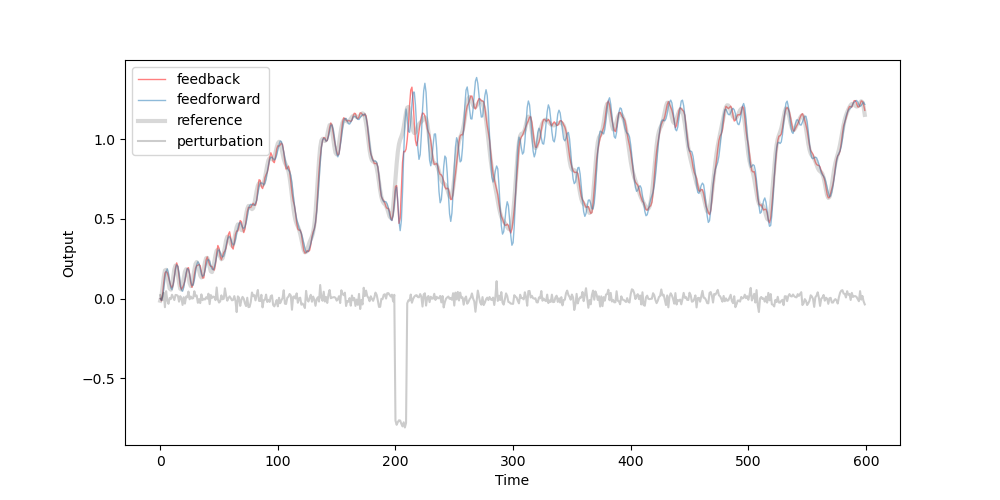
\includegraphics[width=\textwidth]{baseline_linear/fig/MG_lin_noise.png}
    \caption{MG, linear RNN and LQG under perturbation, without onging hebbian learning.}
\end{figure}


\newpage

%%%%%%%

\section*{Week 10/31 - 11/13}

\subsection*{Goal}

\noindent
Main Task: Feedback control in non-linear system under periodic perturbation.

\begin{itemize}
    \item Get extended kalman filter and non-linear LQR to make the gain modulation RNN work under feedback control
    \item Add instant noise onto sustained noise
    \item Test Hebbian learning under noise
\end{itemize}

\noindent
Reading

\begin{itemize}
    \item \url{https://en.wikipedia.org/wiki/Extended_Kalman_filter}
    \item Li, W., \& Todorov, E. (2004). Iterative linear quadratic regulator design for nonlinear biological movement systems. Proceedings of the First International Conference on Informatics in Control, Automation and Robotics, 222–229.
    \item Sober, S. J., \& Brainard, M. S. (2009). Adult birdsong is actively maintained by error correction. Nature Neuroscience, 12(7), 927–931.
    \item Warren, T. L., Tumer, E. C., Charlesworth, J. D., \& Brainard, M. S. (2011). Mechanisms and time course of vocal learning and consolidation in the adult songbird. Journal of Neurophysiology, 106(4), 1806–1821.
    \item Sober, S. J., \& Brainard, M. S. (2012). Vocal learning is constrained by the statistics of sensorimotor experience. Proceedings of the National Academy of Sciences, 109(51), 21099–21103.
\end{itemize}

\newpage

\subsection*{Model}
\begin{itemize}
    \item Structure: 1 input layer (1D input), 1 recurrently-connected hidden layer (128 nodes) where 50\% are excitatory neurons (obeying Dale's law), 1 output layer (1D output).

    \item Activation function: sigmoid function $f(y, u) = \frac{1}{1 + e^{-(g + u)(y - s)}}$, where $y$ is the input activation, $u$ is the control input, $g$ is the gain, and $s$ is the shift. 
    
    \item Equations: 
    \begin{eqnarray}
    \nonumber
    x_{t+1} = f(Wx_t + I_{t}, u_{t}) + w_d \\
    \nonumber
    y_t = Cx_{t} + w_n
    \end{eqnarray}
    
    $x_t$ is the activation, $I_t$ is the input after input layer, $u_t$ is the control input, $w_d$ is the Gaussian processing noise following $N(0,W_d)$, $w_n$ is the Gaussian measurement noise following $N(0,W_n)$, $W$ is the weight matrix, $C$ is set to be identity matrix.

    \item Training: Only SGD on gains and shifts. The same model as Week 10/1-10/16.

    \item Feedback control: extended Kalman filter and nonlinear LQR. The basic idea is to use the Jacobian matrix of $f$ at given $x_t$ to approximate linear system.
    
    \item For both SIN and MG, $Q = 10I$, $R = 0.01I$, $W_d = 0.001I$, $W_n = 0.001I$.

\end{itemize}

\newpage

\subsection*{Periodic Perturbation}

\begin{figure}[H]
    \centering
    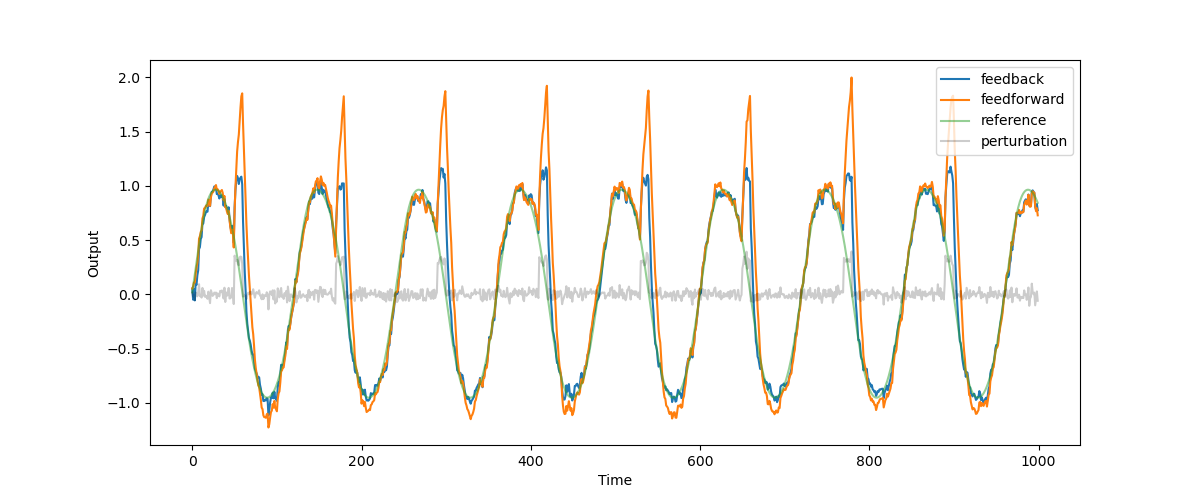
\includegraphics[width=\textwidth]{analysis/fig/1113_SIN_lqg.png}
    \caption{SIN, RNN and LQG on gains under periodic noise, without onging hebbian learning.}
\end{figure}

\begin{figure}[H]
    \centering
    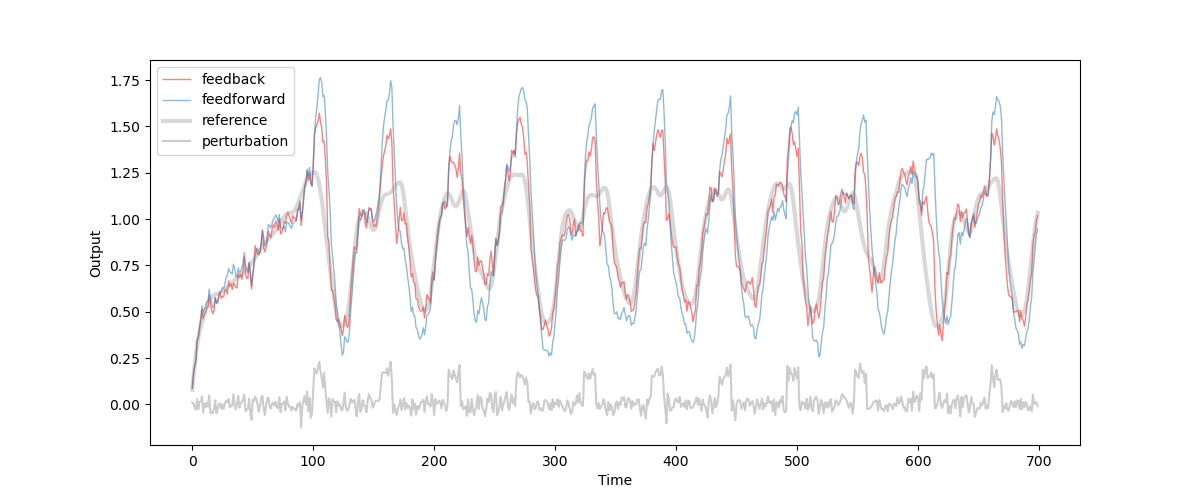
\includegraphics[width=\textwidth]{analysis/fig/1113_MG_lqg.png}
    \caption{MG, RNN and LQG on gains under periodic noise, without onging hebbian learning.}
\end{figure}

\newpage

\subsection*{SIN with Onging Oja Learning}

Oja learning can't ensure a steady performance without noise. The effect of Oja learning is closely related with $\alpha$. When $\alpha$ is large, the regulation term is large, the sum of weights go down making the output go up. When $\alpha$ is small, the regulation term is small, the sum of weights go up making the output go down. Need to investigate how hebbian-like learning could perform stable performance under no error and compensate performance when error occurs.

\newpage

%%%%%%%%

\section*{Week 11/13 - 11/27}

\subsection*{Goal}

\noindent
Main Task: Adaptative gain modulation and feedback control. Learn the perturbation pattern and gradually transfer the learning to synaptic plasticity.

\begin{itemize}
    \item Predictive feedback control: learn to give a control input in advance to correct the periodic perturbation.
    \item Transfer of learning: using Oja learning to transfer the learning effect from gains to synaptic weights.
\end{itemize}

\noindent
Reading

\begin{itemize}
    \item Bittner, K. C., Milstein, A. D., Grienberger, C., Romani, S., \& Magee, J. C. (2017). Behavioral time scale synaptic plasticity underlies CA1 place fields. Science, 357(6355), 1033–1036.
    \item Bouchard, K. E., Ganguli, S., \& Brainard, M. S. (2015). Role of the site of synaptic competition and the balance of learning forces for Hebbian encoding of probabilistic Markov sequences. Frontiers in Computational Neuroscience, 9.
\end{itemize}

\newpage

\subsection*{Predictive Feedback Control Framework}

One possible framework that is able to predictively give control signal to correct periodic perturbation is to use another neural network with Q-learning.

\begin{figure}[H]
    \centering
    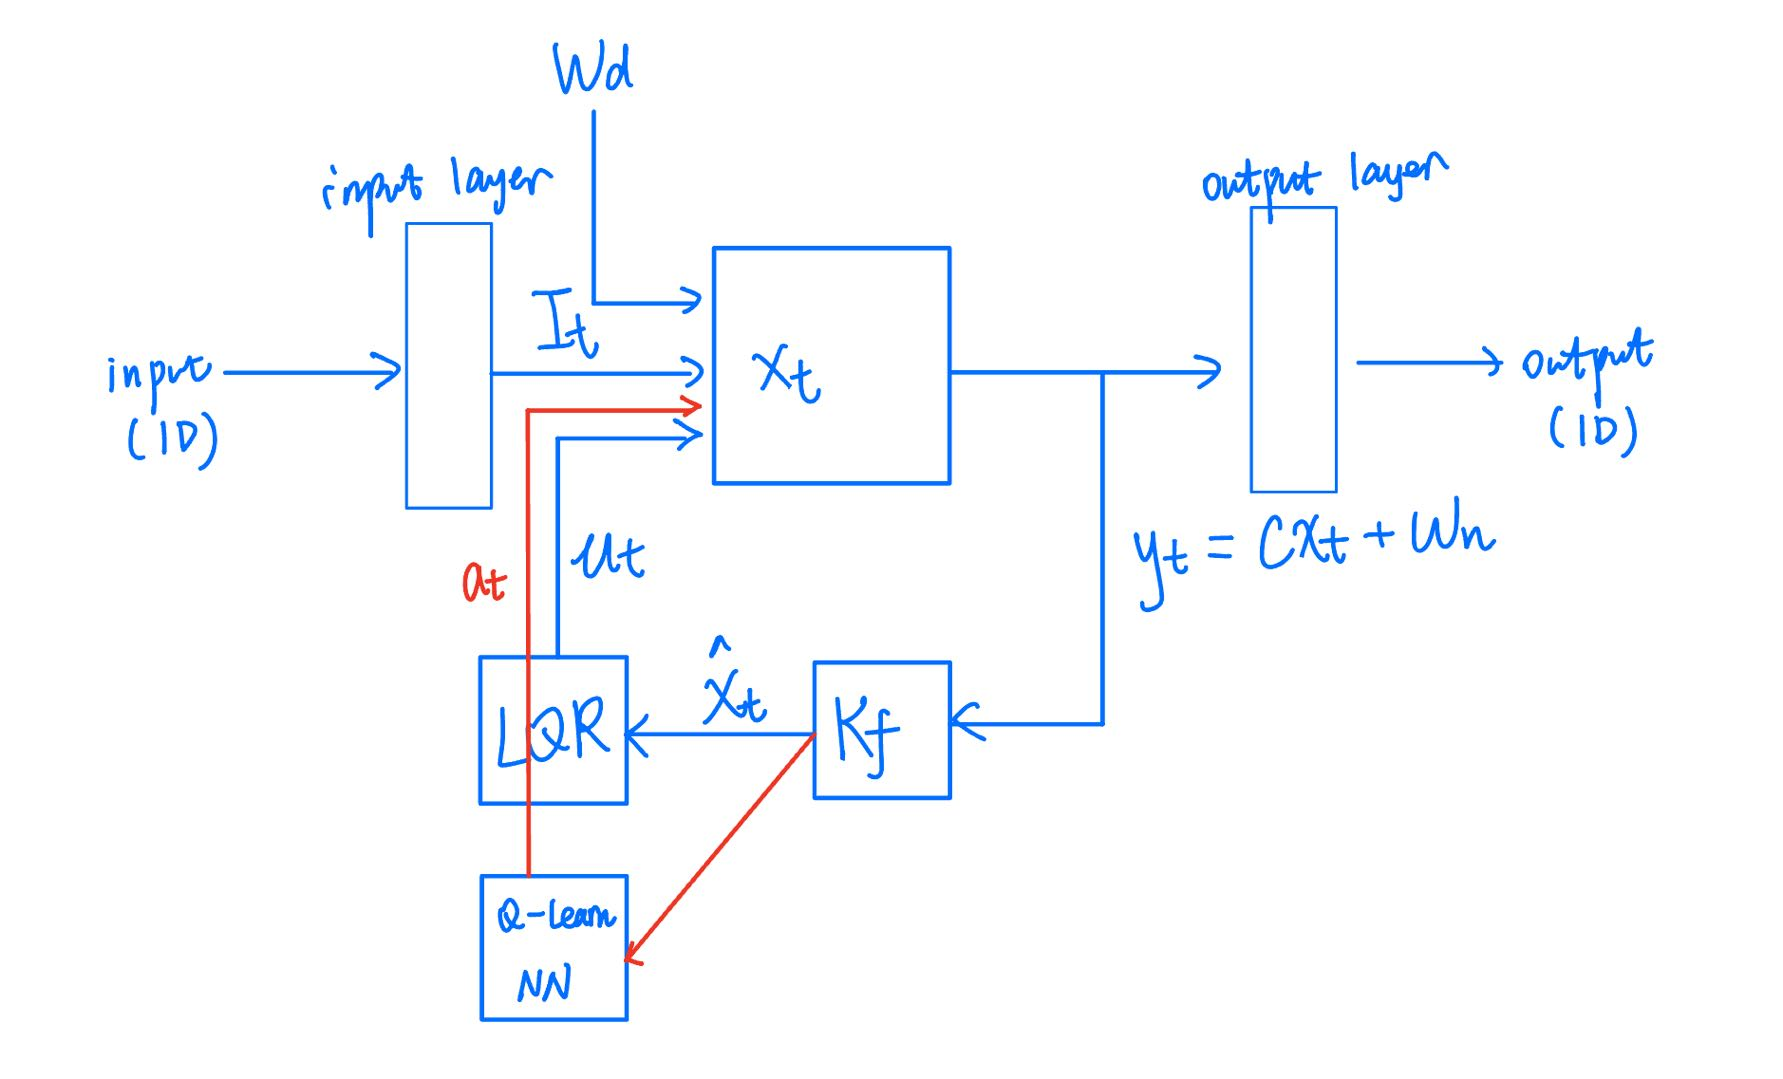
\includegraphics[width=0.8\textwidth]{analysis/fig/qlearn_struc.jpg}
    \label{fig:1}
\end{figure}

Let the state at time $t$ be $x_t$. Given $x_t$, An action $a_t$ (i.e., control signal) could drive the state $x_t$ to some $x_{t+1}$. We define the reward $r_{t+1}$ associate with $x_{t+1}$ as the negative of the distance between the output and the target.

We define the estimated state-action value as $Q(x_t, a_t)$. The goal is to learn the $Q$ function so that it can correctly estimate the future rewards when exert an action $a_t$ at the state $x_t$. Once we have a good $Q$, given $x_t$, we just need to choose $a_t$ that maximize $Q(x_t, a_t)$ as our control signal.

To approximate the function $Q$, we may need to use another simple neural network (since there are infinitely many states and actions), so that $Q(s,a) \approx Q(s,a;\theta)$. The loss function would be 
$$ L = E \left[ \left( r_{t+1} + \gamma \max_{a} Q(s_{t+1},a; \theta) - Q(s_t, a_t; \theta) \right)^2 \right] $$
To simplify, we could assume $\max_{a} Q(s_{t+1}, a; \theta) = 0$, so $ L = E \left[ \left( r_{t+1} - Q(s_t, a_t; \theta) \right)^2 \right] $. 

But training this neural network requires back propagation. Also it would substitute LQR once it is fully functioning.

\newpage

\subsection*{Transfer of Learning}

To explore transfer of learning, I first explore the gains and weights during the initial training (no perturbation). However, it seems that gains are not converging. (By reflection it might be because of Adam optimizer. Shall try SGD later.) Gain change represents the distance between current gains and initial gains. Weight sum represents sum of weights.

I also try to replicate the simple neural network in Swinehart and Abbott (2005), using SGD and Hebbian learning. But it seems that the learning in gains doesn't completely transfer into the weights.

\newpage

%%%%%%%%

\section*{Week 11/27 - 01/22}

\subsection*{Goal}

\noindent
Main Task: Transfer of learning from gains to synapses.

\begin{itemize}
    \item Find out how Swinehart and Abbott (2005) manage to do the transfer of learning
    \item Try hard decay on gain modulation magnitude
    \item Try persistent perturbation rather than periodic perturbation
    \item Slowly grow the Hebbian learning rate, avoid abrupt change
    \item On RNN, try inhibitory synaptic plasticity and get the transfer of learning work
\end{itemize}

\noindent
Reading

\begin{itemize}
    \item Vogels, T. P., Sprekeler, H., Zenke, F., Clopath, C., \& Gerstner, W. (2011). Inhibitory Plasticity Balances Excitation and Inhibition in Sensory Pathways and Memory Networks. Science, 334(6062), 1569–1573.
    \item Vogels, T. P., Froemke, R. C., Doyon, N., Gilson, M., Haas, J. S., Liu, R., Maffei, A., Miller, P., Wierenga, C. J., Woodin, M. A., Zenke, F., \& Sprekeler, H. (2013). Inhibitory synaptic plasticity: Spike timing-dependence and putative network function. Frontiers in Neural Circuits, 7.
    \item Rozell, C., Johnson, D., Baraniuk, R., \& Olshausen, B. (2007). Locally Competitive Algorithms for Sparse Approximation. 2007 IEEE International Conference on Image Processing, IV-169-IV–172.
    \item Paul, A., Wagner, S., \& Das, A. (2022). Learning in Feedback-driven Recurrent Spiking Neural Networks using full-FORCE Training (arXiv:2205.13585). arXiv.
    \item Ogawa, S., Fumarola, F., \& Mazzucato, L. (2023). Multitasking via baseline control in recurrent neural networks. Proceedings of the National Academy of Sciences, 120(33), e2304394120.
\end{itemize}

\newpage

\subsection*{Transfer of Learning in Feedforward Network}

% Last week, I demonstrated a way to transfer learning in gains and shifts to weights. However, it is based on switching hebbian learning on and off frequently: only if the loss for a particular data point is small, hebbian learning is performed. I also actively narrow the gains and shifts boundary. It turns out that it does not work well for RNN or adpatation to perturbation.

Ideally, after doing backprop on gains and shifts, the response tuning curves of side neurons would go up and those of middle neurons would go down. Then, when hebbian learning is turning on, the weights of side neurons would get larger update than those of middle nuerons. Plus, the normalization process would keep the sum of the weights as constant, resulting in a cosine-like weights. The changed weights would "exaggerate" the model outputs (e.g., even lower outputs in the middle of the curve). So, to reduce the loss, The next rounds of backprop would flatten the response tuning curves. In theory, this process transfers the learning in gains and shifts to weights. (We don't really need to actively shrink of gains and shifts by putting a shrinking boundaries. In fact, if the shrinkage/flattening goes too fast, hebbian learning could not result in enough curvature in weights.)

\begin{figure}[H]
    \centering
    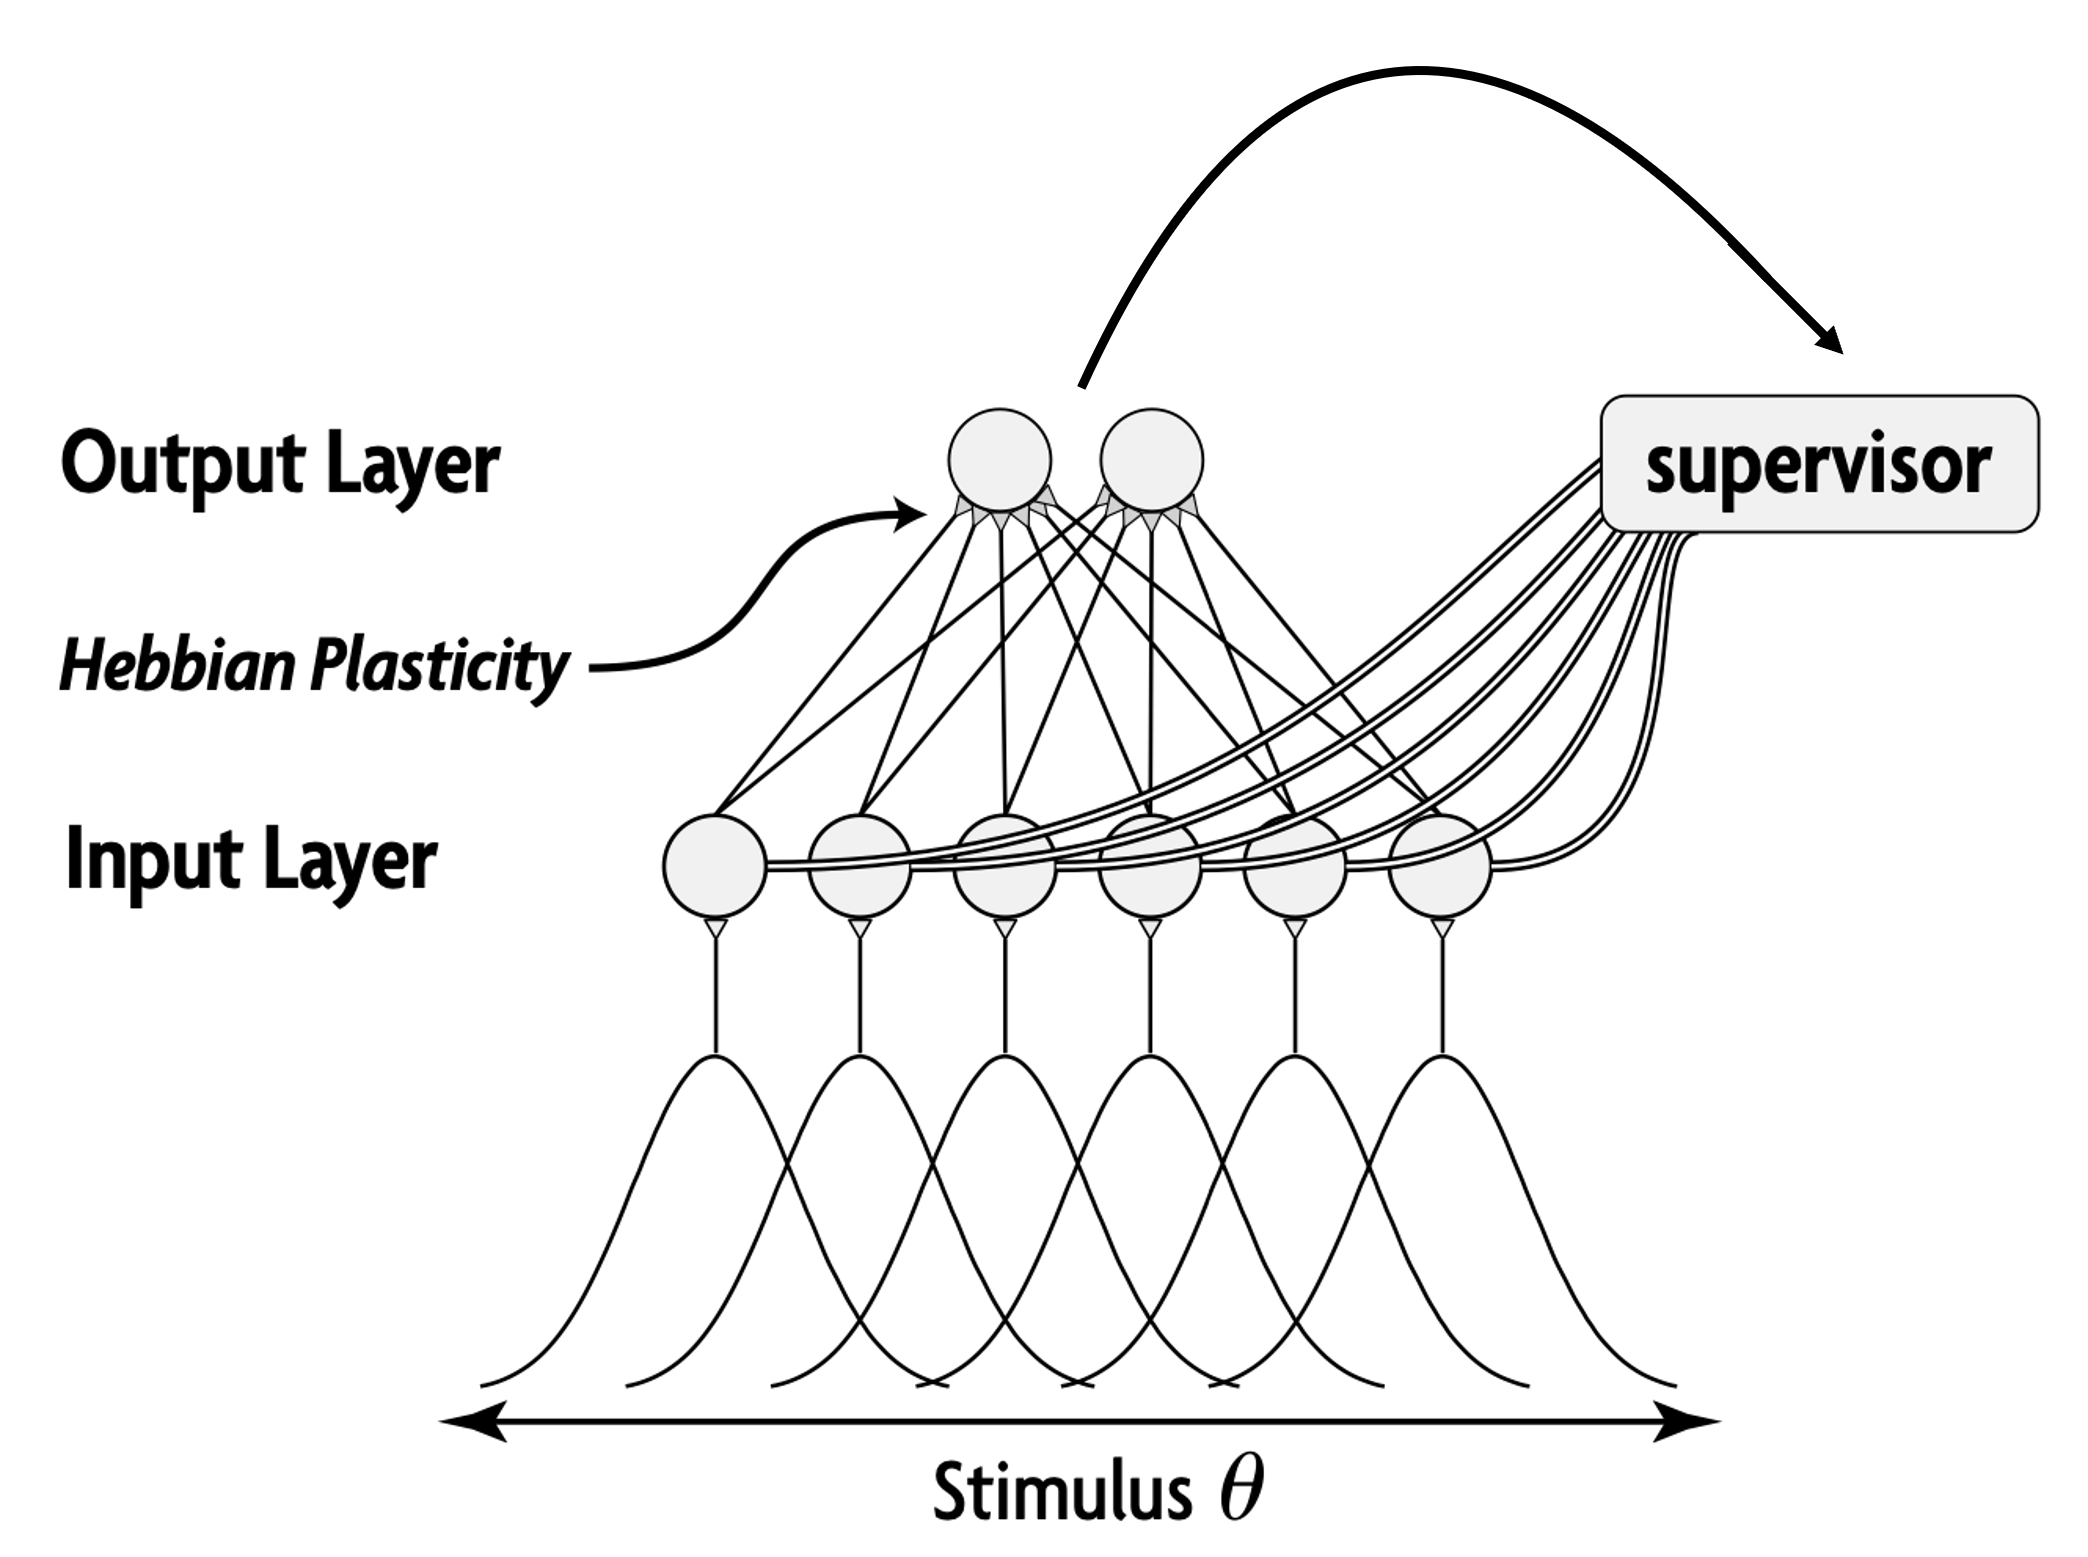
\includegraphics[width=0.45\textwidth]{baseline_abb05/fig/abb05_struc.png}
    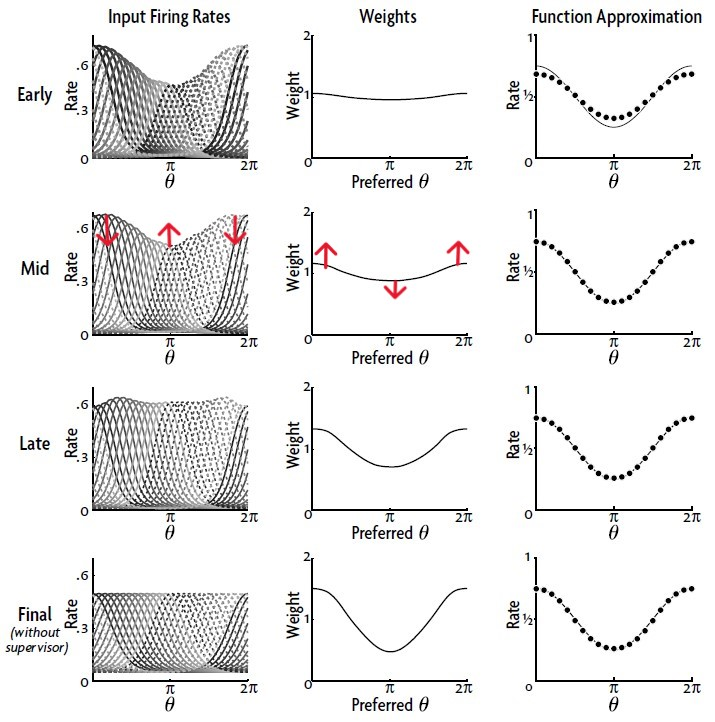
\includegraphics[width=0.45\textwidth]{baseline_abb05/fig/abb05_paperresult_draw.jpg}
    \\
    \caption{The sturcture and the claimed result in the paper.}
\end{figure}

In practice, the process could not transfer the learning completely, returning the gains and shifts to the initial values. It would converge to a state where the learning is partly in weights and partly in gains and shifts. 

\begin{figure}[H]
    \centering
    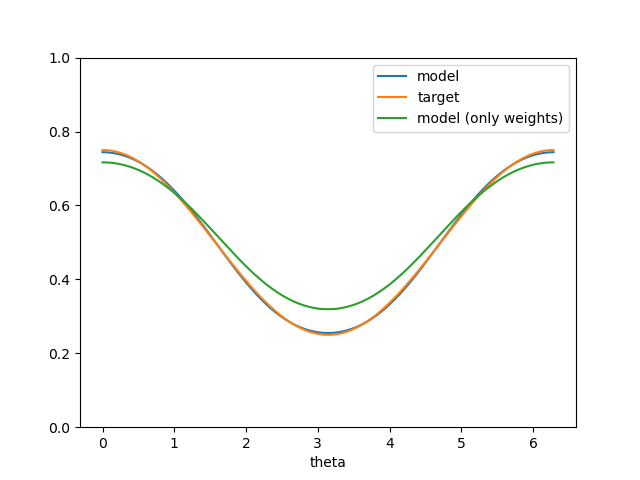
\includegraphics[width=0.3\textwidth]{baseline_abb05/fig/0122_abb05_bphebb_onlyweights.png}
    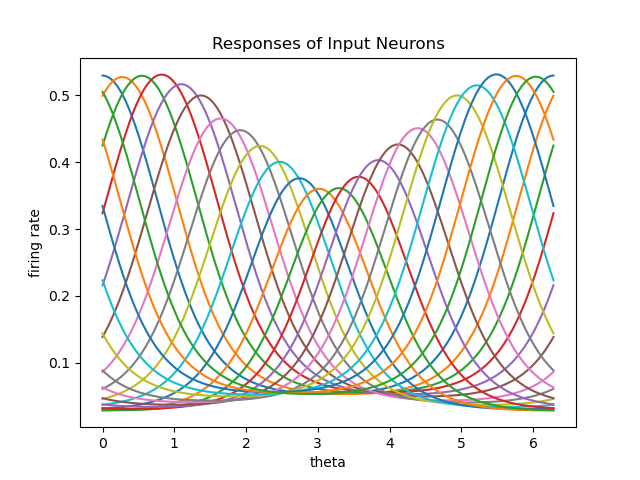
\includegraphics[width=0.3\textwidth]{baseline_abb05/fig/0122_abb05_bphebb_rf.png}
    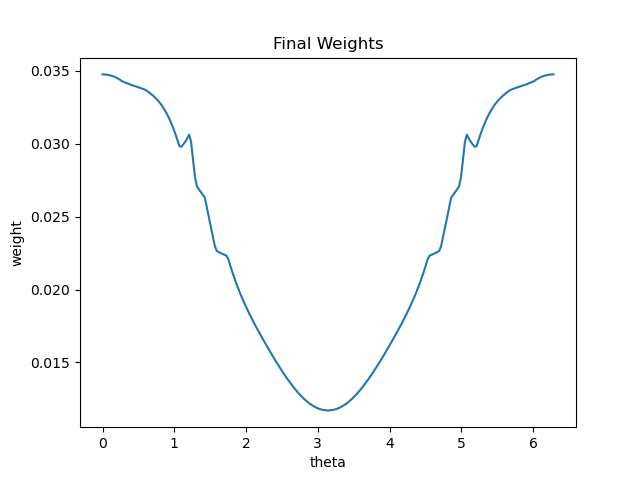
\includegraphics[width=0.3\textwidth]{baseline_abb05/fig/0122_abb05_bphebb_weights.png}
    \\
    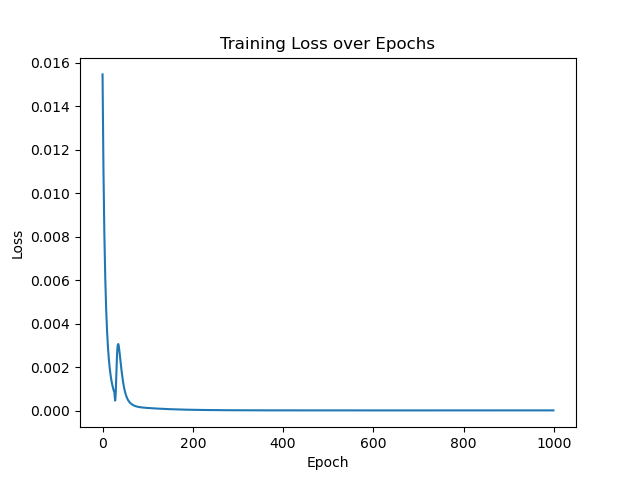
\includegraphics[width=0.3\textwidth]{baseline_abb05/fig/0122_abb05_bphebb_loss.png}
    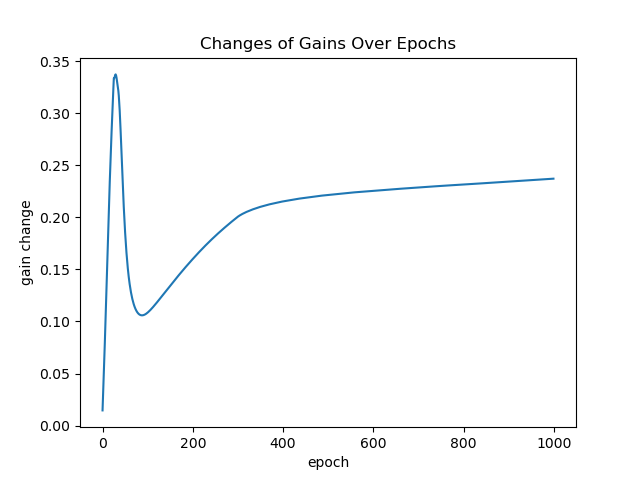
\includegraphics[width=0.3\textwidth]{baseline_abb05/fig/0122_abb05_bphebb_gc.png}
    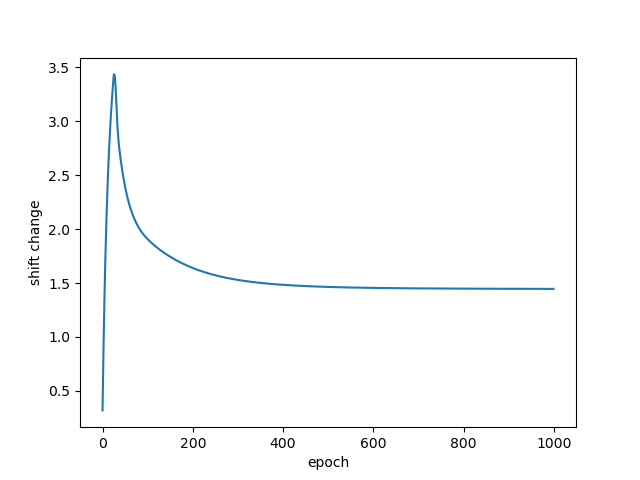
\includegraphics[width=0.3\textwidth]{baseline_abb05/fig/0122_abb05_bphebb_sc.png}\\
    \caption{Hebbian learning start after 10 epoches.}
\end{figure}

To understand this, I did an experiment where I keep the gains and shifts unchanged as initial and use backprop to find the "correct" weights. Then I turn on the hebbian learning, but the "correct" weights is not stable. In fact, it would converge to some weights whose loss is high. In other words, the "correct" weights is not a convergence point of hebbian learning.

\begin{figure}[H]
    \centering
    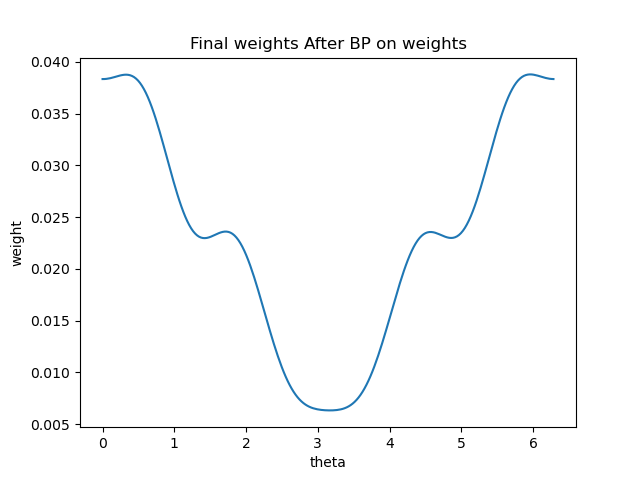
\includegraphics[width=0.45\textwidth]{baseline_abb05/fig/0122_abb05_wt_weights.png}
    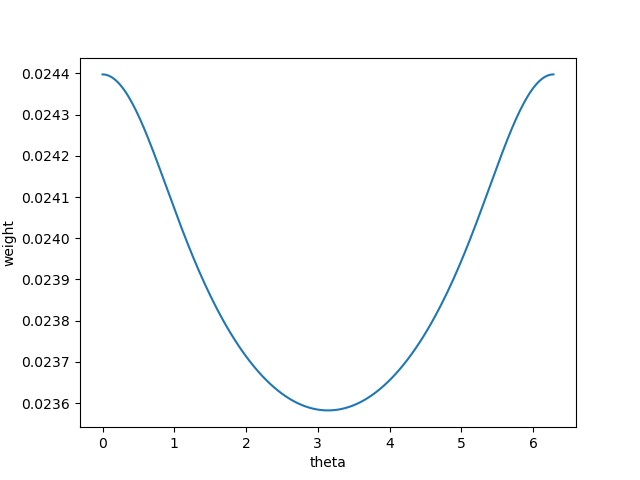
\includegraphics[width=0.45\textwidth]{baseline_abb05/fig/0122_abb05_wtconv_loss.png} \\
    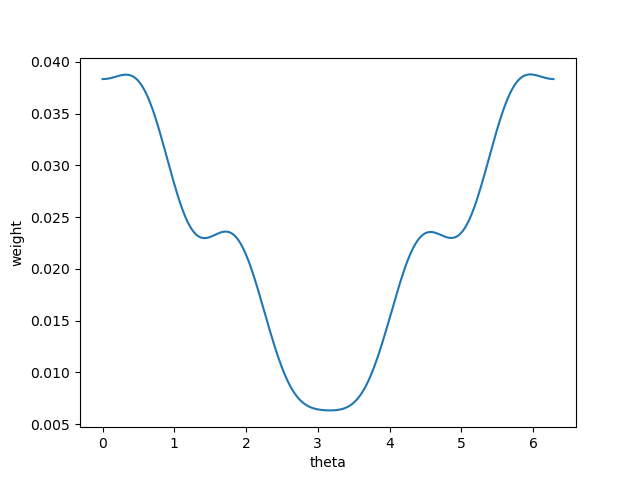
\includegraphics[width=0.45\textwidth]{baseline_abb05/fig/0122_abb05_wtconv_weights.png}
    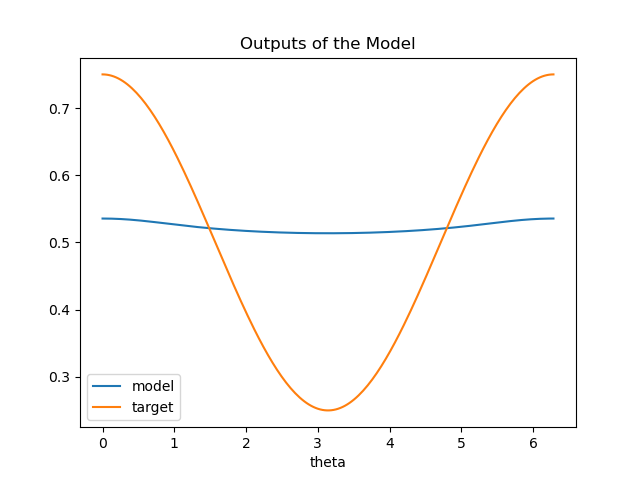
\includegraphics[width=0.45\textwidth]{baseline_abb05/fig/0122_abb05_wtconv_output.png}
    \caption{Changes after Hebbian learning on initial gains and correct weights.}
\end{figure}

Mathemetically, the convergence point of hebbian learning should meet some requirements. Say, there are $n$ input nodes and $m$ inputs. For the $i$th input, the activation of input nodes are $a_{i1},\dots,a_{in}$. The target output is $y_i$. Let $w_j$ be the weight from $j$th input nodes to the output node. Denote matrix $A={a_{ij}}$, vector $y=(y_1,\dots,y_n)^T$, vector $w=(w_1,\dots,w_n)^T$. So the "correct" weights should satisfy: $$Aw=y$$
The hebbian update before normalization to the weights would be $A^Ty$. If the weights are to remain the same, the hebbian update should be in the same direction as original weights: $$A^Ty=kw$$
This leads us to $A^TAw=kw$, meaning that only if the "correct" weights are eigenvectors of $A^TA$ could hebbian learning converge.

\subsection*{Perturbation in Feedforward Network}

After the network is trained, I try to add a persistent deviation in neurons' activation after 50 epoches, The perturbation lasts for 1000, 2000, or 5000 epoches. From the losses one could see, the network adapts to the perturbation quickly (with both backprop and hebbian learning), and after the perturbation is turned off, the loss goes up suddenly but gradually goes back to normal.

\begin{figure}[H]
    \centering
    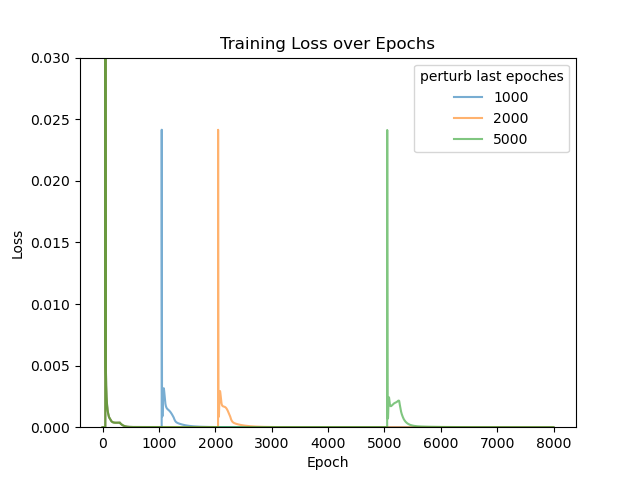
\includegraphics[width=0.45\textwidth]{baseline_abb05/fig/0122_abb05_perturb_loss.png} \\
    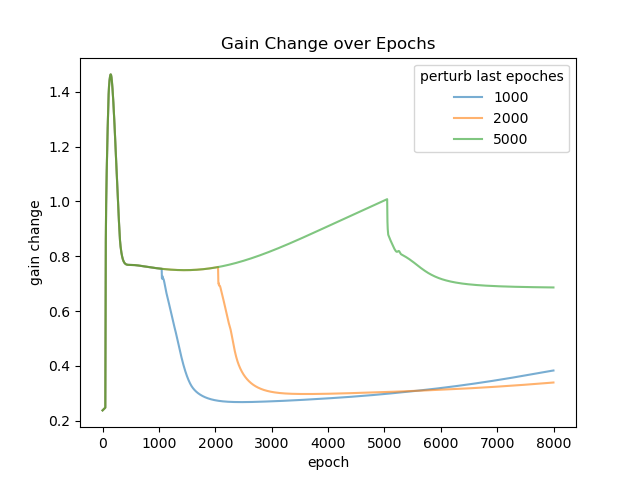
\includegraphics[width=0.45\textwidth]{baseline_abb05/fig/0122_abb05_perturb_gc.png} 
    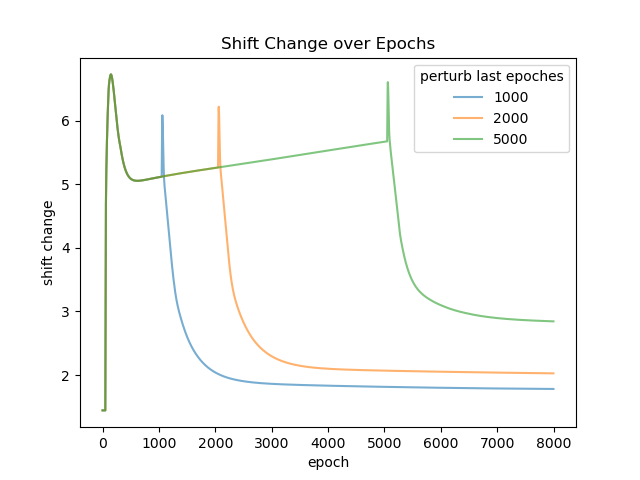
\includegraphics[width=0.45\textwidth]{baseline_abb05/fig/0122_abb05_perturb_sc.png}
    \caption{Perturbation in feedforward netork.}
\end{figure}

\newpage

\subsection*{Transfer of learning in RNN}

I implement the same training paradigm to train the RNN, i.e., first do backprop on gains and shifts and then turn on hebbian learning, to see how much of the learning could be transfered from gains and shifts to weights.

Some details: 32 nodes in recurrent layer; hebbian learning is performed for every timestep; evenly distributed gaussian receptive fields for each neuron; output weight matrix are set to all 1 and -1; one epoch represents 1 period of sinwave with 120 timesteps.

For inhibitory synaptic plasticity, I didn't find a principle applicable for firing rate network. Existing attempts are all based on spike timings. So I just use the same idea as in excitatory synapses: the more they are firing together, the inhibitory synapses are stronger (more negative).

\begin{figure}[H]
    \centering
    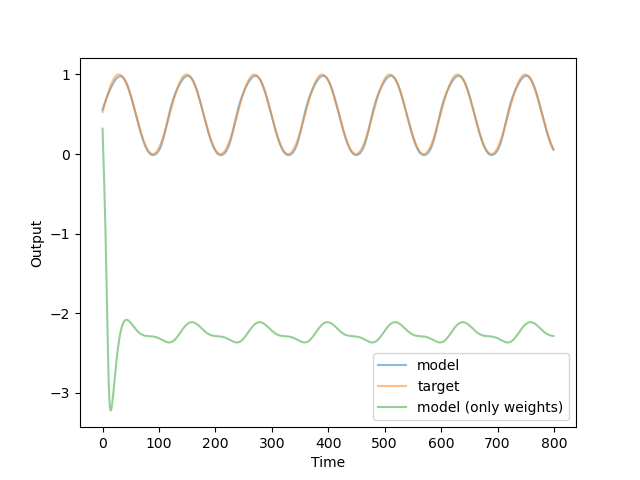
\includegraphics[width=0.3\textwidth]{analysis/fig/0122_SIN2_bphebbpt_output.png}
    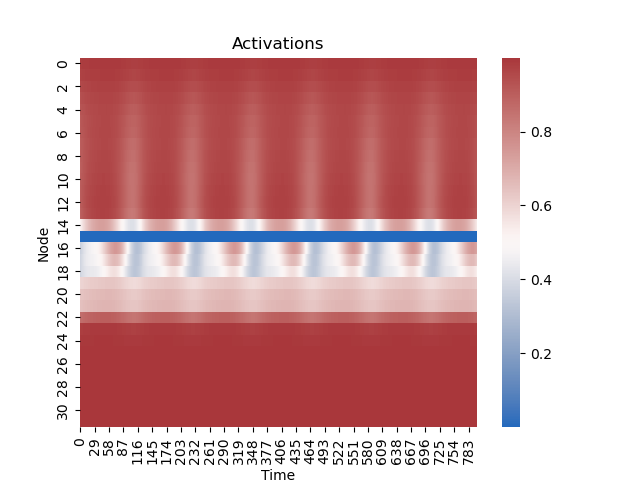
\includegraphics[width=0.3\textwidth]{analysis/fig/0122_SIN2_bphebbpt_activations.png}
    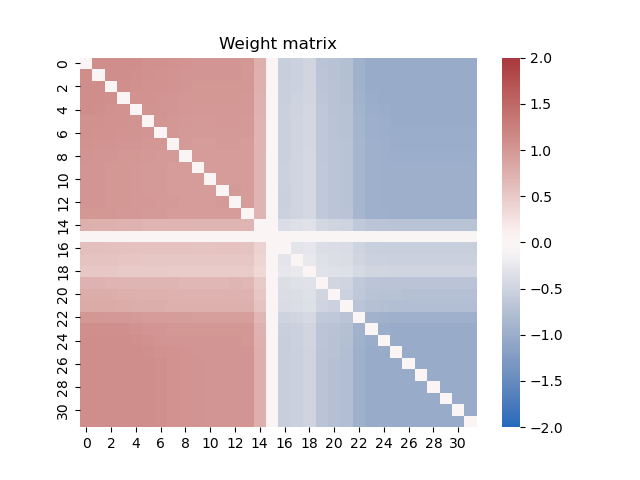
\includegraphics[width=0.3\textwidth]{analysis/fig/0122_SIN2_bphebbpt_weight_matrix.png}\\
    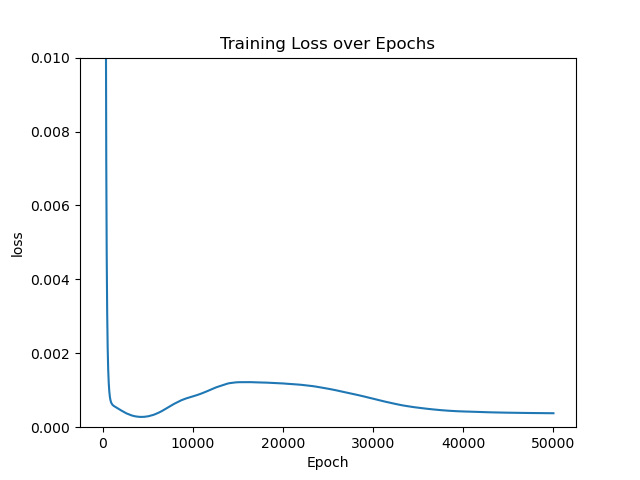
\includegraphics[width=0.3\textwidth]{analysis/fig/0122_SIN2_bphebbpt_loss.png}
    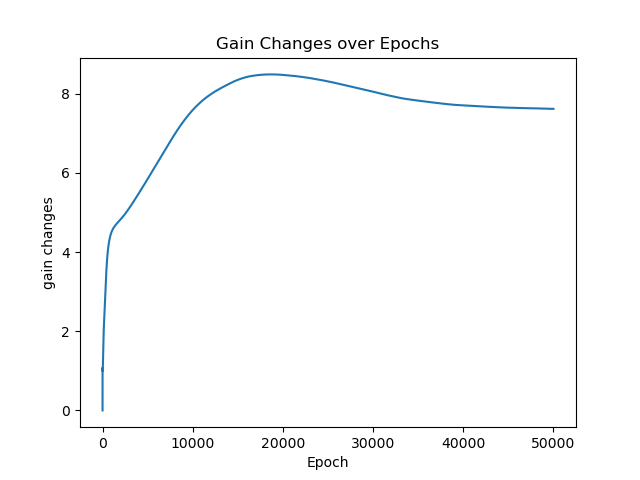
\includegraphics[width=0.3\textwidth]{analysis/fig/0122_SIN2_bphebbpt_gc.png}
    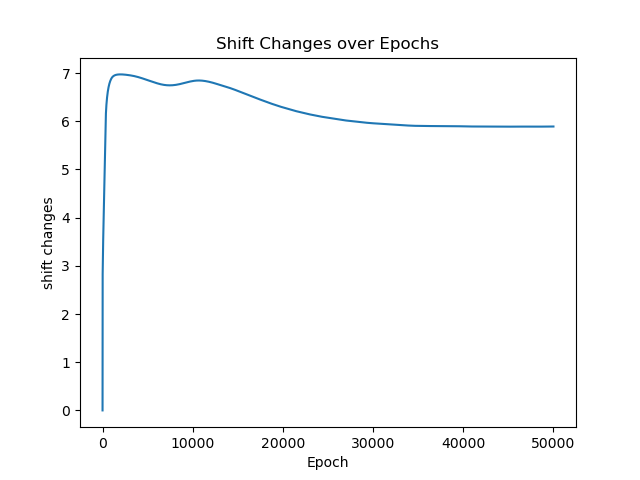
\includegraphics[width=0.3\textwidth]{analysis/fig/0122_SIN2_bphebbpt_sc.png}\\
    \caption{Hebbian learning start after 1000 epoches.}
\end{figure}

Notice the grid-like weights after hebbian learning. It is quite different from the "correct" weights obtained from backprop on weights.

\begin{figure}[H]
    \centering
    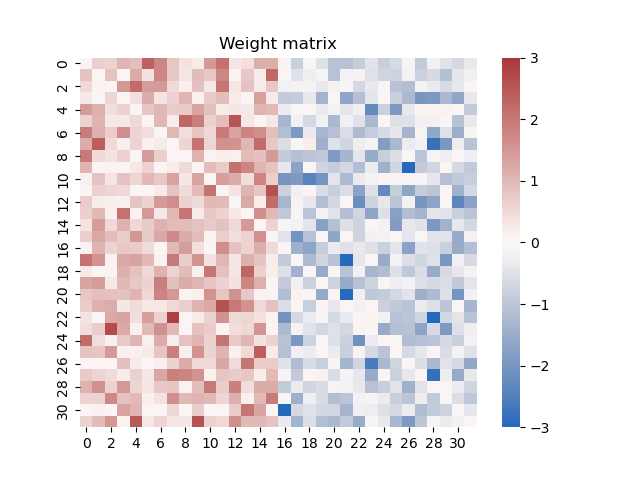
\includegraphics[width=0.45\textwidth]{analysis/fig/0122_SIN2_wt_weight_matrix.png}
    \caption{Weight matrix after backprop on weights.}
\end{figure}

\subsection*{Perturbation in RNN}

After the network is trained, I try to add a persistent deviation in the input after 50 epoches, The perturbation lasts for 2000, 5000, or 10000 epoches.

\begin{figure}[H]
    \centering
    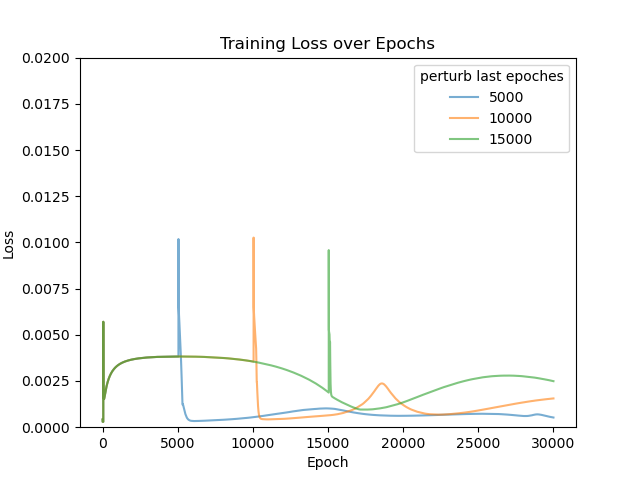
\includegraphics[width=0.6\textwidth]{analysis/fig/0122_SIN2_perturb_loss.png} \\
    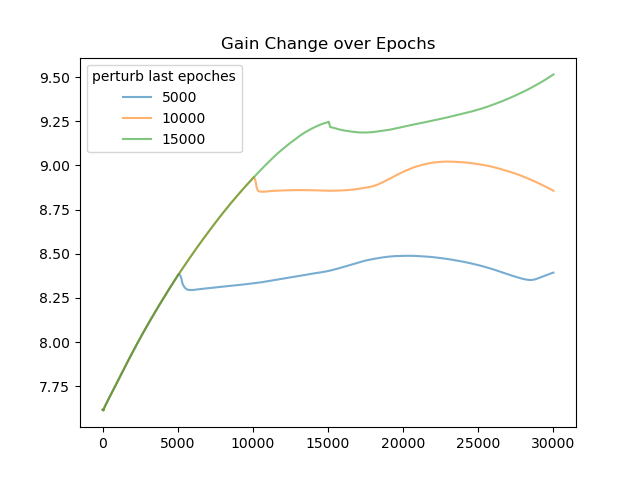
\includegraphics[width=0.45\textwidth]{analysis/fig/0122_SIN2_perturb_gc.png} 
    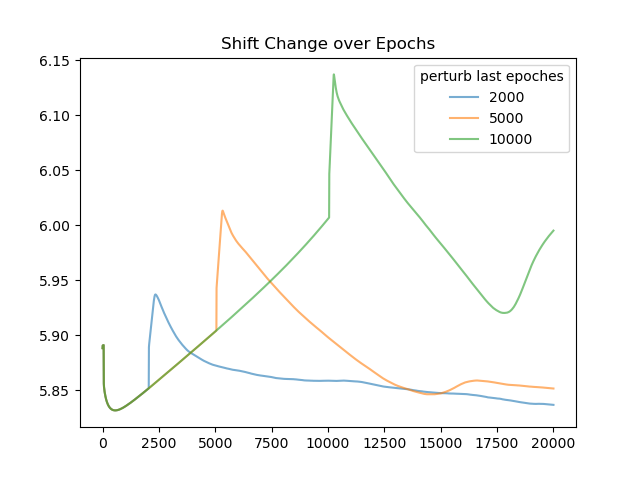
\includegraphics[width=0.45\textwidth]{analysis/fig/0122_SIN2_perturb_sc.png}
    \caption{Perturbation in RNN.}
\end{figure}

\subsection*{Thoughts}

\begin{itemize}
    \item Hebbian learning may not be able to transfer all the learning from gains and shifts to weights. Hebbian learning is after all unsupervised learning, especially in RNN, how could $n$ nodes instruct $n^2$ weights to learn?
    \item How to change backprop to feedback control is another problem. As our RNN is trained with backprop and it is backprop that reaches a balance with hebbian learning, it is hard for feedback control to reach a similar balance. Primitive attempt reveals that hebbian learning would cause the output drift away under feedback control.
    \item A plausible inhibitory synapses learning rule is yet to find. Maybe we should try on building the spiking neural network?
\end{itemize}

\newpage

%%%%%%%

\section*{Week 01/22 - 02/20}

\subsection*{Goal}

\noindent
Main Task: Transfer of learning from gains to synapses.

\begin{itemize}
    \item Get the transfer of learning feedforward network work. Try to look at the scale of weights.
    \item Systematically investigate the adaptation to perturbation.
    \item Think of a better way to implement hebbian learning in RNN, especially inhibitory hebbian learning.
\end{itemize}

\noindent
Reading

\begin{itemize}
    \item Bouchard, K. E., Ganguli, S., \& Brainard, M. S. (2015). Role of the site of synaptic competition and the balance of learning forces for Hebbian encoding of probabilistic Markov sequences. Frontiers in Computational Neuroscience, 9.
    \item Rajan, K., \& Abbott, L. F. (2006). Eigenvalue Spectra of Random Matrices for Neural Networks. Physical Review Letters, 97(18), 188104.
    \item Murphy, B. K., \& Miller, K. D. (2009). Balanced Amplification: A New Mechanism of Selective Amplification of Neural Activity Patterns. Neuron, 61(4), 635–648.
    \item Oja, E. (1982). Simplified neuron model as a principal component analyzer. Journal of Mathematical Biology, 15, 267--273.
    \item Hennequin, G., Agnes, E. J., \& Vogels, T. P. (2017). Inhibitory Plasticity: Balance, Control, and Codependence. Annual Review of Neuroscience, 40(1), 557–579.
\end{itemize}

\newpage

\subsection*{Transfer of Learning in Feedforward Network}

We were facing the scaling problem last week that the weights and the outputs have a correct cosine shape but not the correct value. I scrutinized but couldn't find any difference between my code and Swinehart's code. So at last, I tuned and changed the gain and shift of the output node, from gain = 3 and shift = 1 to gain = 6.67 and shift = 1.035 (after all, there is nothing special about 3 and 1). These parameters are selected so that Hebbian learning could converge at the correct value given the input nodes have initial gains and shifts and the output node has target activation.

Below are more training details:
\begin{itemize}
    \item Two layers. 230 Input nodes. 1 Output nodes. Model stucture is shown in Figure 7.
    \item The input nodes have gaussian receptive field for different stimulus value determining the input current $I_i$, and sigmoid activation function $r_i = \frac{1}{1 + e^{-g_i(I_i-s_i)}}$, where initially gain $g_i = 3$ and shift $s_i = 1$. $g_i$ and $s_i$ could be adjusted during training.
    \item The output node is connected to input nodes through weights $w_i$, and has sigmoid activation function $r_o = \frac{1}{1 + e^{-g_o(\sum w_ir_i - s_o)}}$, where gain $g_i = 6.67$ and shift $s_i = 1.035$.
    \item The task is to approximate a cosine function. For the supervisor, we use squared error loss and SGD on gains and shifts of input nodes with learning rate = 0.2.
    \item Hebbian learning is applied to weights, $w_i \rightarrow w_i + \eta r_i r_o$, where $\eta$ gradually increase from 0 until reaching maximum = 0.0001 at 80th epoch. After each update there is also a normalization step to keep all the weights sum to 5.5.
    \item A passive boundary at gains and shifts are applied starting from 20th epoch, that is, in the following epoch the gains and shifts could only be more closed to the initial value than the current epoch.
\end{itemize}

In this way, we make the transfer of learning work.

% figures of bphebb

\newpage

\subsection*{Perturbation in Feedforward Network}

We want to test whether the network would show some adaptation effect if undergoing a period of persistent perturbation. Using the trained network, we keep the simulation going, add a persistent noise to all input nodes at 50th epoch ($r_i = \frac{1}{1 + e^{-g_i(I_i-s_i) + \epsilon_i}}$, $\epsilon_i \sim N(1,0.001)$), last for certain epochs, and then turn off.

We systemetically control the perturbation lasting to investigate the adaptation effect. To quantify the adaptation, we define two indices to represent the "difficulty" for the network to recover after perturbation: (1) area under the loss curve (AUC) and (2) how many epochs it takes to return to loss $<$ 0.0001. The results show that the longer the perturbation lasts, the harder for a network to recover. And we also observe a tendency of saturation.

% fig of perturb

We also control the magnitude of perturbation. Here we fix the duration of perturbation as 500 epochs, but change the mean amplitude of noise, i.e., $\epsilon_i \sim N(x, 0.001)$. We find that, if the amplitude of perturbation is too large, the network would fail to learn or reduce its loss under perturbation, and thus recover quickly when the perturbation is turned off. The failure of learning under large perturbation is due to saturation in sigmoid function and thus the gradient vanishes.

% fig of amp

\subsection*{Some Attemps in RNN}


\end{document}